\begin{example}[Proposition 9 : $n = 6, \mathcal{PF'}_n \to \mathcal{D}_n$]
    ~\
    \begin{itemize}
        \item $f = (1, 1, 2, 4, 5, 5)$
            \subitem $l_1 = 2$
            \hspace{2cm} $l_2 = 1$
            \hspace{2cm} $l_3 = 0$
            \subitem $l_4 = 1$
            \hspace{2cm} $l_5 = 2$
            \hspace{2cm} $l_6 = 0$
        \item $w = (110100101100)$
    \end{itemize}
    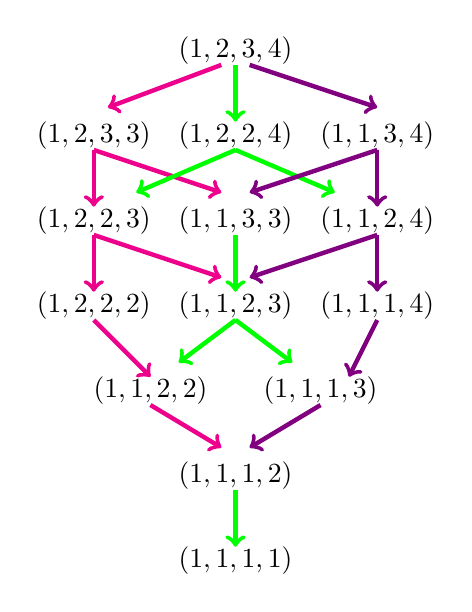
\begin{tikzpicture}[scale = 0.18]
    \node at (0,0)   {$(1,1,1,1)$};
    \node at (0,6)   {$(1,1,1,2)$};                
    \node at (-6,12) {$(1,1,2,2)$};
    \node at (6,12)  {$(1,1,1,3)$};
    \node at (-10,18) {$(1,2,2,2)$};
    \node at (0,18)  {$(1,1,2,3)$};
    \node at (10,18)  {$(1,1,1,4)$};
    \node at (-10,24) {$(1,2,2,3)$};
    \node at (0,24)  {$(1,1,3,3)$};
    \node at (10,24)  {$(1,1,2,4)$};
    \node at (-10,30) {$(1,2,3,3)$};
    \node at (0,30)  {$(1,2,2,4)$};
    \node at (10,30)  {$(1,1,3,4)$};
    \node at (0,36)  {$(1,2,3,4)$};


    \draw [->][color=magenta, ultra thick] (-1,35) to (-9,32);
    \draw [->][color=magenta, ultra thick](-10,29) to (-10,25);
    \draw [->][color=magenta, ultra thick](-10,29) to (-1,26); 
    \draw [->][color=magenta, ultra thick](-10,23) to (-10,19);
    \draw [->][color=magenta, ultra thick](-10,23) to (-1,20);
    \draw [->][color=magenta, ultra thick](-10,17) to (-6,13);
    \draw [->][color=magenta, ultra thick](-6,11) to (-1,8);


    \draw [->][color=green, ultra thick](0,35) to (0,31);
    \draw [->][color=green, ultra thick](0,29) to (-7,26);
    \draw [->][color=green, ultra thick](0,29) to (7,26);
    \draw [->][color=green, ultra thick](0,23) to (0,19);
    \draw [->][color=green, ultra thick](0,17) to (-4,14);
    \draw [->][color=green, ultra thick](0,17) to (4,14);
    \draw [->][color=green, ultra thick](0,5) to (0,1);

    \draw [->][color=violet, ultra thick](1,35) to (10,32);
    \draw [->][color=violet, ultra thick](10,29) to (1,26);
    \draw [->][color=violet, ultra thick](10,29) to (10,25);
    \draw [->][color=violet, ultra thick](10,23) to (1,20);
    \draw [->][color=violet, ultra thick](10,23) to (10,19);
    \draw [->][color=violet, ultra thick](10,17) to (8,13);
    \draw [->][color=violet, ultra thick](6,11) to (1,8);

\end{tikzpicture}
\end{example}

\begin{example}[Proposition 9 : $n = 6, \mathcal{D}_n \to \mathcal{PF'}_n$]
    ~\
    \begin{itemize}
        \item $w = 101011010010$
    \end{itemize}
        \begin{center}
        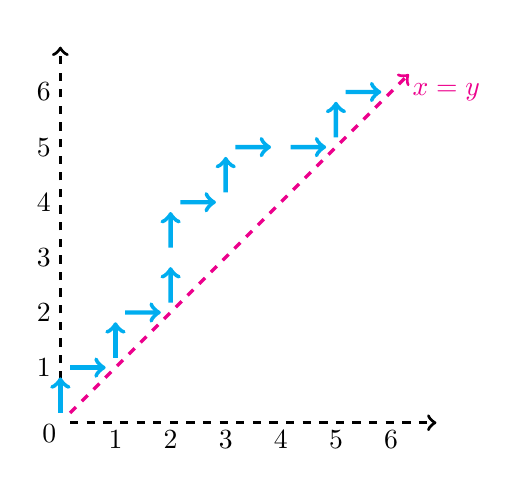
\begin{tikzpicture}[scale=0.7]
            \node (a) at (0, 0) {};
            \node (b) at (0, 7) {};
            \node (c) at (7, 0) {};
            \node (d) at (6.5, 6.5) {};
            \node (e) at (7, 6) [color = magenta]
                {$x = y$}; 
            \draw [dashed, very thick, ->] (a) to (b);
            \draw [dashed, very thick, ->] (a) to (c);
            \draw [dashed, very thick, ->]
                [color = magenta] (a) to (d);

            \node (1)  at (0,0)   {};
            \node (2)  at (0,1)   {};
            \node (3)  at (1,1)   {};
            \node (4)  at (1,2)   {};
            \node (5)  at (2,2)   {};
            \node (6)  at (2,3)   {};
            \node (7)  at (2,4)   {};
            \node (8)  at (3,4)   {};
            \node (9)  at (3,5)   {};
            \node (10) at (4,5)   {};
            \node (11) at (5,5)   {};
            \node (12) at (5,6)   {};
            \node (13) at (6,6)   {};
            \draw [->, ultra thick, color = cyan]
                (1)  to (2);
            \draw [->, ultra thick, color = cyan] 
                (2)  to (3);
            \draw [->, ultra thick, color = cyan]
                (3)  to (4);
            \draw [->, ultra thick, color = cyan]
                (4)  to (5);
            \draw [->, ultra thick, color = cyan]
                (5)  to (6);
            \draw [->, ultra thick, color = cyan]
                (6)  to (7);
            \draw [->, ultra thick, color = cyan]
                (7)  to (8);
            \draw [->, ultra thick, color = cyan]
                (8)  to (9);
            \draw [->, ultra thick, color = cyan]
                (9)  to (10);
            \draw [->, ultra thick, color = cyan]
                (10) to (11);
            \draw [->, ultra thick, color = cyan]
                (11) to (12);
            \draw [->, ultra thick, color = cyan]
                (12) to (13);

            \node at (-0.2, -0.2) {$0$};
            \node at (-0.3, 1)    {$1$};
            \node at (1, -0.3)    {$1$};
            \node at (-0.3, 2)    {$2$};
            \node at (2, -0.3)    {$2$};
            \node at (-0.3, 3)    {$3$};
            \node at (3, -0.3)    {$3$};
            \node at (-0.3, 4)    {$4$};
            \node at (4, -0.3)    {$4$};
            \node at (-0.3, 5)    {$5$};
            \node at (5, -0.3)    {$5$};
            \node at (-0.3, 6)    {$6$};
            \node at (6, -0.3)    {$6$};

        \end{tikzpicture}
    \end{center}
    \begin{itemize}
        \item Distances : 
            \subitem $s_1 = 0$
                \hspace{2cm} $a_1 = 1$
            \subitem $s_2 = 1$
                \hspace{2cm} $a_2 = 2$
            \subitem $s_3 = 2$
                \hspace{2cm} $a_3 = 3$
            \subitem $s_4 = 2$
                \hspace{2cm} $a_4 = 3$
            \subitem $s_5 = 3$
                \hspace{2cm} $a_5 = 4$
            \subitem $s_6 = 5$
                \hspace{2cm} $a_6 = 6$
        \item $f = (1, 2, 3, 3, 4, 6)$
    \end{itemize}
    
\end{example}

\begin{example}[Définition 10 : $n = 7$]
    $10110011001100 \gtrdot_d 10110101001100$
    \begin{itemize}
        \item $w_1 = 10110$
        \item $w_2 = 1001100$
    \end{itemize}
    \input{fig/fig6.tex}
\end{example}

\begin{example}[Définition 13 : $n = 6$]
    $(1, 1, 2, 3, 4, 5) \gtrdot (1, 1, 2, 3, 3, 5)$    
\end{example}

\begin{example}[Proposition 15 : $n = 6, \mathcal{PF}_n \to \mathcal{LD}_n$]
    ~\
    \begin{itemize}
        \item $f = (5, 2, 1, 4, 5, 1)$
            \subitem $im_1 = \{3, 6\}$
            \hspace{16mm} $im_2 = \{2\}$
            \hspace{24mm} $im_3 = \emptyset$
            \subitem $im_4 = \{4\}$
            \hspace{2cm} $im_5 = \{1, 5\}$
            \hspace{2cm} $im_6 = \emptyset$
        \item $w = 360200401500$
    \end{itemize}
    \input{fig/fig8.tex}
\end{example}

\begin{example}[Proposition 15 : $n = 6, \mathcal{LD}_n \to \mathcal{PF}_n$]
    ~\
    \begin{itemize}
        \item $w = 402560010030$
    \end{itemize}
    \input{fig/fig9.tex}
    \begin{itemize}
        \item Distances :
            \subitem $s_1 = 0$
            \hspace{2cm} $s_2 = 1$
            \hspace{2cm} $s_3 = 1$
            \subitem $s_4 = 1$
            \hspace{2cm} $s_5 = 3$
            \hspace{2cm} $s_6 = 5$
        \item Labels :
            \subitem $dist_0 = \{4\}$
            \hspace{2cm} $dist_1 = \{2, 5, 6\}$
            \hspace{2cm} $dist_2 = \emptyset$
            \subitem $dist_3 = \{1\}$
            \hspace{2cm} $dist_4 = \emptyset$
            \hspace{32mm} $dist_5 = \{3\}$
        \item $f = (4, 2, 6, 1, 2, 2)$
    \end{itemize}
\end{example}

\begin{example}[Définition 16 : $n = 5$]
    $104503600200 \gtrdot_{ld} 10345060200$
    ~\\
    \begin{itemize*}
        \item $l = 10$
        \item $r = 0200$
        \item $x = 45$
        \item $x' = 345$
        \item $y = 3$
        \item $z = 36$
        \item $z' = 6$
    \end{itemize*}
    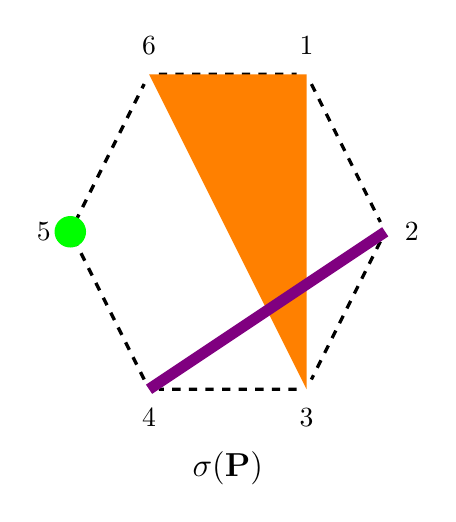
\begin{tikzpicture}[scale=1]
    \node at (3,0) {\large $\mathbf{\sigma (P)}$};
    \node [label = above : {$1$}] (1)
        at (4,5) {};
    \node [label = right : {$2$}] (2)
        at (5,3) {};
    \node [label = below : {$3$}] (3)
        at (4,1) {};
    \node [label = below : {$4$}] (4)
        at (2,1) {};
    \node [label = left : {$5$}]  (5)
        at (1,3) {};
    \node [label = above : {$6$}] (6)
        at (2,5) {};
    \draw [dashed][very thick]
    (1) -- (2) -- (3) -- (4)
        -- (5) -- (6) -- (1);
    \fill [color = orange] (4,5) -- (4,1)
        -- (2,5) -- cycle;
    \draw [color = violet][line width = 4pt] 
        (5,3) -- (2,1);
    \fill [color=green] (1,3) circle (0.2);
    
  \end{tikzpicture}
\end{example}

\begin{example}[Définition 17 : $n = 5$]
    Dans l'ordre, les montées de $104503600200$ sont :\\
    \begin{itemize*}
        \item $1$
        \item $45$
        \item $36$
        \item $\emptyset$
        \item $2$
        \item $\emptyset$
    \end{itemize*}
\end{example}